\subsection*{Matrix Assembly Loops}
\begin{frame}[fragile,t]  
%  \frametitle{Poisson Equation}
	\begin{block}{}
	  \begin{itemize}    
	  \item{ The \libmesh{} representation of the matrix and
	    rhs assembly is similar to the mathematical statements.
	  }
	  \end{itemize}
	\end{block}
\small
\begin{semiverbatim}
for (q=0; q<Nq; ++q) 
  for (i=0; i<Ns; ++i) \{
    \alert<2>{Fe(i)   += \alert<3>{JxW[q]}*\alert<4>{f(xyz[q])}*\alert<5>{phi[i][q]};}
    
    for (j=0; j<Ns; ++j)
      \alert<6>{Ke(i,j) += \alert<7>{JxW[q]}*(\alert<8>{dphi[j][q]*dphi[i][q]});}
  \}
\end{semiverbatim}
\only<2-5>
{
  \begin{equation}
    \nonumber
    \bv{F}^e_{i} = 
    \sum_{q=1}^{N_q}
    \alert<4>{f(x(\xi_q))}
    \alert<5>{\phi_i(\xi_q)}
    \alert<3>{|J(\xi_q)| w_q}
  \end{equation}
}
\only<6->
{
  \begin{equation}
  \nonumber
  \bv{K}^e_{ij} =
  \sum_{q=1}^{N_q}
  \alert<8>{
    \hat{\nabla}_{\!\xi} \phi_j(\xi_q) \cdot
    \hat{\nabla}_{\!\xi} \phi_i(\xi_q)
    }
  \alert<7>{|J(\xi_q)| w_q}
  \end{equation}
}
\end{frame}


\begin{frame}[allowframebreaks]
  \lstinputlisting[basicstyle=\tiny\ttfamily]{snippets/poisson_eqn.cxx}
\end{frame}
 

\frame
{
  \Large
  \begin{block}{}
    \center{\bf A Complete Program:}
    \center{\texttt{poisson\_ex1}}
  \end{block}
}



\begin{frame}[fragile]
  \frametitle{Poisson class definition}

  \begin{lstlisting}
// headers omitted for brevity
class Poisson : public System::Assembly
{
public:
  Poisson (EquationSystems &es_in) :
    es (es_in)
  {}

  void assemble ();

  Real exact_solution (const Real x,
                       const Real y,
                       const Real z = 0.) const
  {
    static const Real pi = acos(-1.);

    return cos(.5*pi*x)*sin(.5*pi*y)*cos(.5*pi*z);
  }

private:
  EquationSystems &es;
};
  \end{lstlisting}
\end{frame}


\begin{frame}[allowframebreaks]
  \frametitle{Poisson \texttt{main()}}
  \lstinputlisting[basicstyle=\tiny\ttfamily]{tutorial/poisson_ex1/main.C}
\end{frame}


\begin{frame}[allowframebreaks]
  \frametitle{Poisson \texttt{assembly()}}
  \lstinputlisting[basicstyle=\tiny\ttfamily]{tutorial/poisson_ex1/poisson_problem.C}
\end{frame}


\begin{frame}[fragile]
  \frametitle{Running the program}
    \begin{block}{Running the program}
    \begin{lstlisting}[language=bash]
# copy the example

$ make

# run the example in 2D with 20 elements in each direction
$ ./example-opt -d 2 -n 20 

# run the example in 3D with 20 elements in each direction
$ ./example-opt -d 3 -n 20 
    \end{lstlisting}
  \end{block}
\end{frame}

\frame
{
  \frametitle{Output}
  \begin{center}
    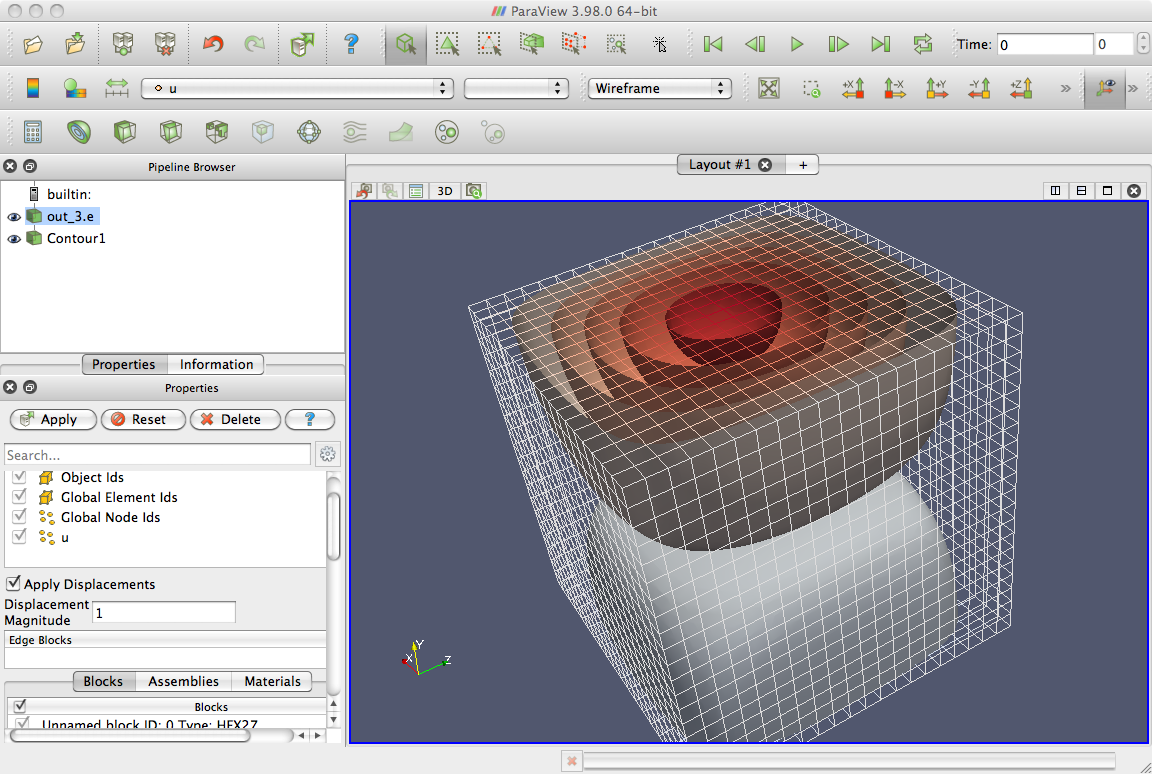
\includegraphics[height=0.8\textheight]{tutorial/poisson_ex1/screen}
  \end{center}
} 

\frame
{
  \Large
  \begin{block}{}
    \center{\bf Extension: Multithreaded Assembly:}
    \center{\texttt{poisson\_threaded}}
  \end{block}
}



\begin{frame}[fragile,shrink]
  \frametitle{Poisson class definition}

  \begin{lstlisting}
// headers omitted for brevity
class Poisson : public System::Assembly
{
public:
  Poisson (EquationSystems &es_in) :
    es (es_in)
  {}

  void assemble ();

  void operator()(const ConstElemRange &range) const;

  Real exact_solution (const Real x,
                       const Real y,
                       const Real z = 0.) const
  {
    static const Real pi = acos(-1.);

    return cos(.5*pi*x)*sin(.5*pi*y)*cos(.5*pi*z);
  }

private:
  EquationSystems &es;

  mutable Threads::spin_mutex assembly_mutex;
};
  \end{lstlisting}
\end{frame}



\begin{frame}[fragile,shrink]
  \frametitle{Threaded Poisson assembly}

  \begin{lstlisting}
#include "poisson_problem.h"

void Poisson::assemble ()
{
  const MeshBase& mesh = es.get_mesh();

  ConstElemRange assembly_elem_range (mesh.active_local_elements_begin(),
                                      mesh.active_local_elements_end());

  Threads::parallel_for (// the range over which we will perform threaded operations
                         assembly_elem_range,

                         // the function object to apply to each element in the range
                         *this);
}

void Poisson::operator()(const ConstElemRange &range) const
{
  ...

  // insert the local (per-thread) element matrix/vector into
  // the global matrix/vector.  This is a shared object, so we
  // must be careful to lock for exclusive access.
  {
    Threads::spin_mutex::scoped_lock lock(assembly_mutex);
    
    system.matrix->add_matrix (Ke, dof_indices);
    system.rhs->add_vector    (Fe, dof_indices);
  }
}
  \end{lstlisting}
\end{frame}
\begin{frame}[fragile]
  \frametitle{Running the program}
    \begin{block}{Running the program}
    \begin{lstlisting}[language=bash]
# copy the example

$ make

# run the example in 2D with 20 elements in each direction
$ ./example-opt -d 2 -n 20 

# run the example in 3D with 20 elements in each direction
# using various numbers of threads
$ ./example-opt -d 3 -n 20 --n_threads=1
$ ./example-opt -d 3 -n 20 --n_threads=2
$ ./example-opt -d 3 -n 20 --n_threads=4

    \end{lstlisting}
  \end{block}
\end{frame}
